\appendix
\chapter{Advanced software topics}
\section{Creating FPGA and XML files}
\subsection{Create FPGA target and XML}\label{subsec:Create-FPGA-target}
If you do not have a Veristand FPGA target at your disposal, follow the steps below. If you have a target available and just need to install it in NI Veristand, please jump to Section \ref{sec:install_FPGA_in_veristand}. For CS Enterprise 1 and CS Arctic Drill Ship, the FPGA targets are found on GitHub. 
\begin{enumerate}
	\item Open LabVIEW and create new project. In this guide, LabVIEW 2013 is used, but the procedure should be similar on newer versions. 
	\item Choose NI Veristand FPGA Project in project templates and proceed.
	\item Choose CompactRIO Reconfiguarble Embedded System and click next.
	\item You will now get the choice between letting LabVIEW detect your cRIO  system or configure it yourself. If you are connected to the cRIO and it has all of the I/O ports connected, the option ``Discover existing system'' is simpler and therefore recommneded. If you do not have your cRIO connected choose ``Create new system'', this is the version that will be worked through here.
	\item Select your controller, in our case cRIO-9024.
	\item Select your FPGA target, in our case cRIO-9113.
	\item Then you select your I/O modules to the correct slots. In our case NI 9215 in slot 1 and NI 9474 in slot 4.
	\item You are now finished with configuring your project. Press next.
	\item The project menu will now appear and should look something like Figure
	\ref{fig: Create Labview FPGA target and XML-10}. Select the LabVIEW VI as demonstrated our is called Custom Personality FPGA.vi
	\item The UI window will now present itself, select window and show block diagram.
	\item You should now see a block diagram similar to Figure \ref{fig: Create Labview FPGA target and XML-11}. You will now have to redesign this to look like Figure \ref{fig: Create Labview FPGA target and XML-12}. This will be valid for our system, if you have different I/O modules the block diagram need to reflect this.
	\item Now, return to the Project explorer and select Build Specifications and Custom Personality FPGA
	\item A new window will open. Check that the name and project path is correct and press build.
	\item Select your preferred compile server. The compilation process will take quite some time (approx 15-30 min).
	\item When the compilation process is finished, the last step is to edit the automatically generated XML file. You will now have to find you project directory in Windows. Here there will be a folder called bitfiles which contains the files you compiled in the last step, there will also be a .XML file. The point of editing this file is to match the actually compiled VI, meaning the packets must match the connected I/O. The recommended way to edit the file is to copy our XML file from: Dropbox\textbackslash{}TMR4243 - LAB\textbackslash{}04 cRIO software\textbackslash{}FPGA IO. You will have to make sure that the name of your bitfile matches the name in the XML file as seen in Figure \ref{fig: Create Labview FPGA target and XML-17}, also make sure the I/O modules matches your setup.
	\item Copy the bitfiles from the bitfile folder to the level above so that the bitfile aand the XML file is in the same folder.
\end{enumerate}
Documentation: \url{https://decibel.ni.com/content/docs/DOC-13815}

\begin{figure}[htb!]
	\centering 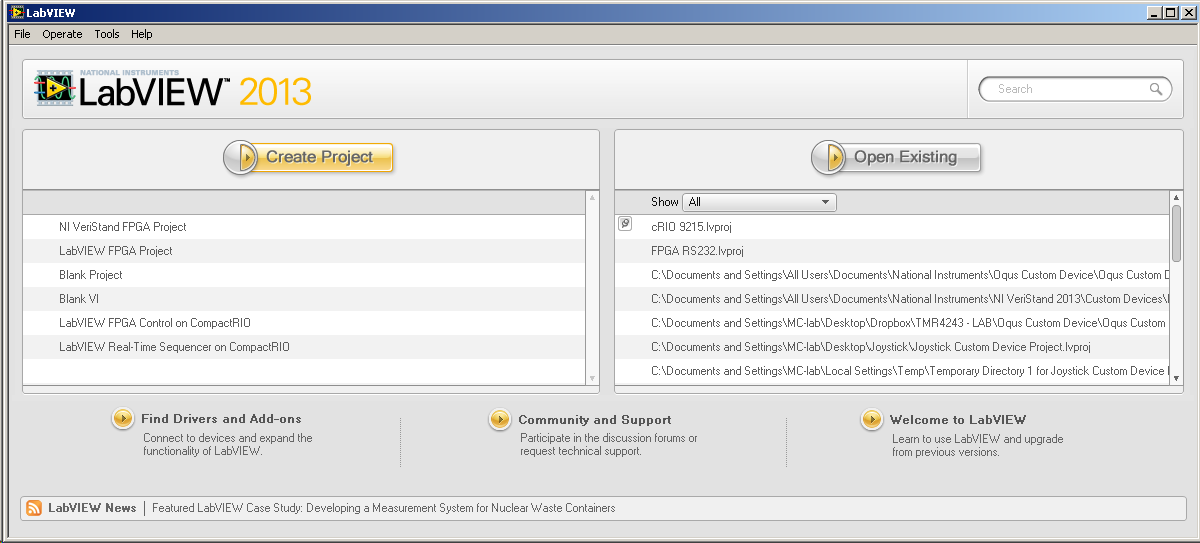
\includegraphics[scale=0.45]{Screenshots/Screenshot_2015-01-16_19-21-16.png}
	\caption{Create Labview FPGA target and XML - 1}
	\label{fig: Create Labview FPGA target and XML-1} 
\end{figure}
\begin{figure}[htb!]
	\centering 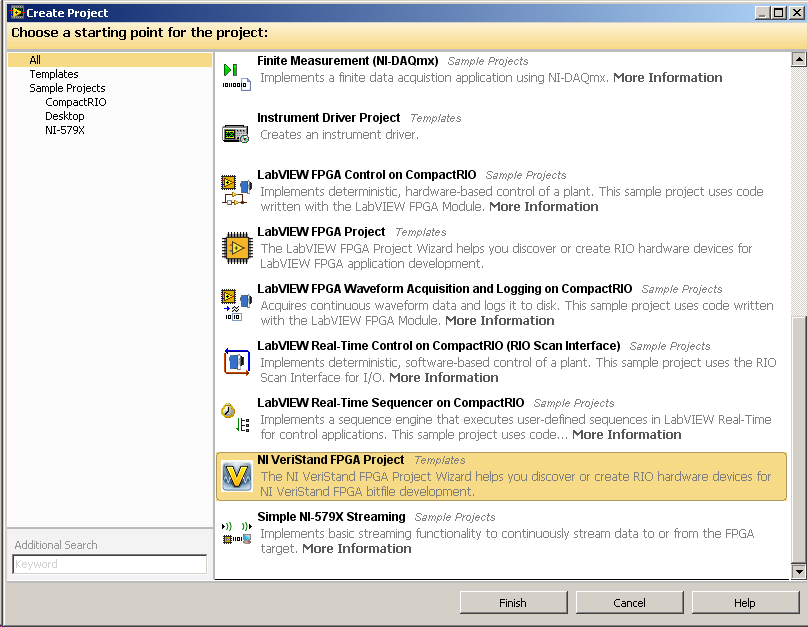
\includegraphics[scale=0.45]{Screenshots/Screenshot_2015-01-16_19-23-23.png}
	\caption{Create Labview FPGA target and XML - 2}
	\label{fig: Create Labview FPGA target and XML-2} 
\end{figure}
\begin{figure}[htb!]
	\centering 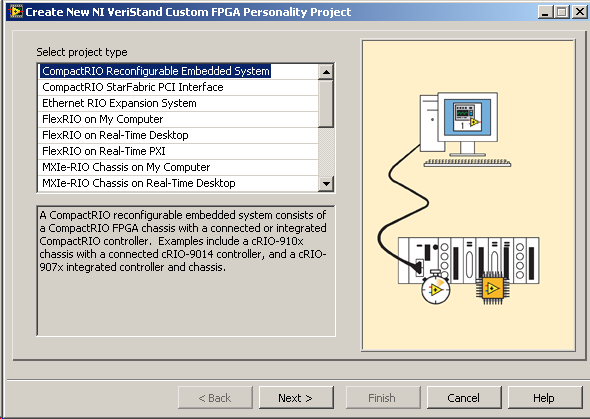
\includegraphics[scale=0.45]{Screenshots/Screenshot_2015-01-16_19-23-41.png}
	\caption{Create Labview FPGA target and XML - 3}
	\label{fig: Create Labview FPGA target and XML-3} 
\end{figure}
\begin{figure}[htb!]
	\centering 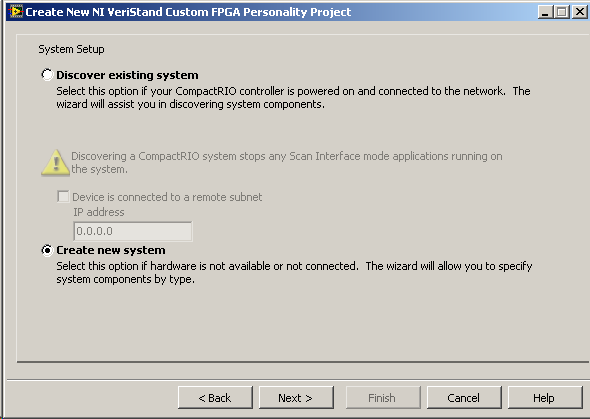
\includegraphics[scale=0.45]{Screenshots/Screenshot_2015-01-16_19-23-58.png}
	\caption{Create Labview FPGA target and XML -4}
	\label{fig: Create Labview FPGA target and XML-4} 
\end{figure}
\begin{figure}[htb!]
	\centering 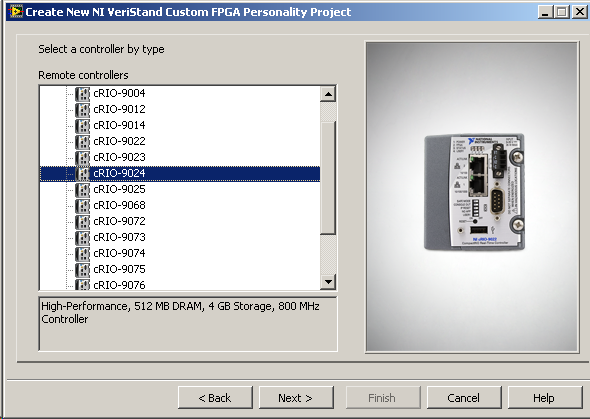
\includegraphics[scale=0.45]{Screenshots/Screenshot_2015-01-16_19-24-31.png}
	\caption{Create Labview FPGA target and XML - 5}
	\label{fig: Create Labview FPGA target and XML-5} 
\end{figure}
\begin{figure}[htb!]
	\centering 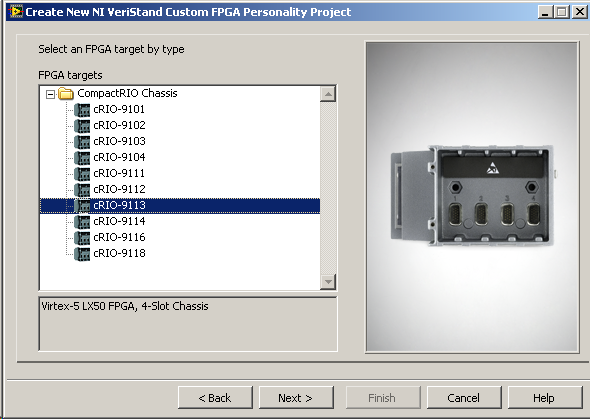
\includegraphics[scale=0.45]{Screenshots/Screenshot_2015-01-16_19-24-43.png}
	\caption{Create Labview FPGA target and XML - 6}
	\label{fig: Create Labview FPGA target and XML-6} 
\end{figure}
\begin{figure}[htb!]
	\centering 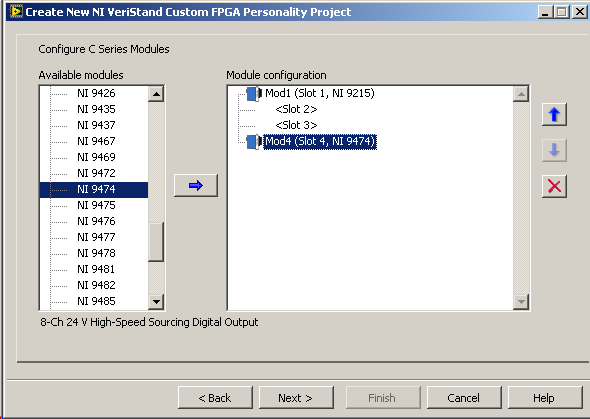
\includegraphics[scale=0.45]{Screenshots/Screenshot_2015-01-16_19-25-37.png}
	\caption{Create Labview FPGA target and XML - 7}
	\label{fig: Create Labview FPGA target and XML-7} 
\end{figure}
\begin{figure}[htb!]
	\centering 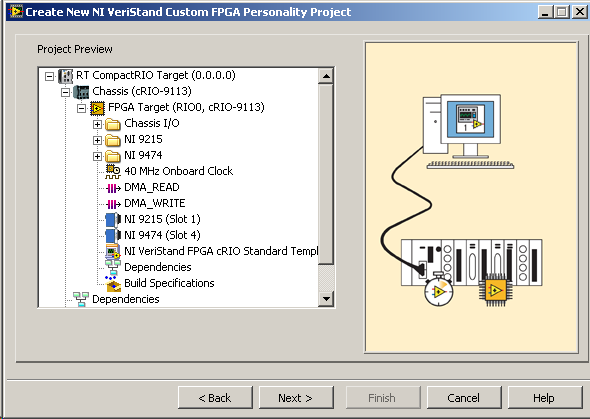
\includegraphics[scale=0.45]{Screenshots/Screenshot_2015-01-16_19-25-54.png}
	\caption{Create Labview FPGA target and XML - 8}
	\label{fig: Create Labview FPGA target and XML-8} 
\end{figure}
\begin{figure}[htb!]
	\centering 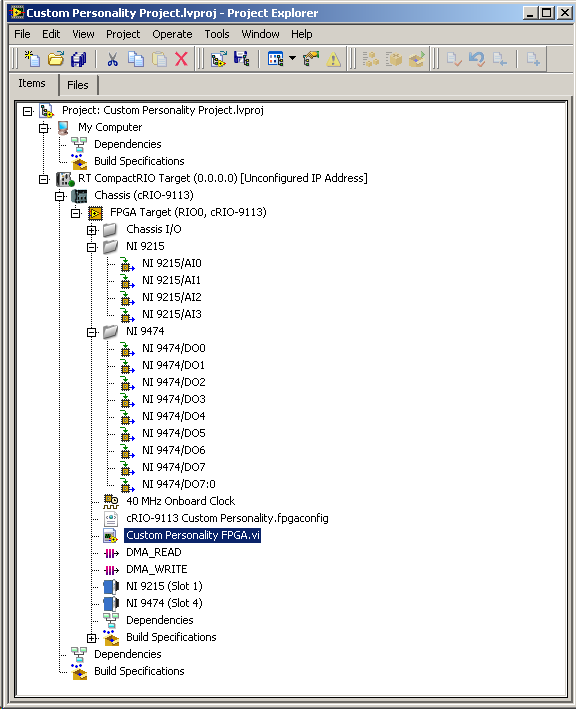
\includegraphics[scale=0.45]{Screenshots/Screenshot_2015-01-16_19-28-17.png}
	\caption{Create Labview FPGA target and XML -9}
	\label{fig: Create Labview FPGA target and XML-9} 
\end{figure}
\begin{figure}[htb!]
	\centering 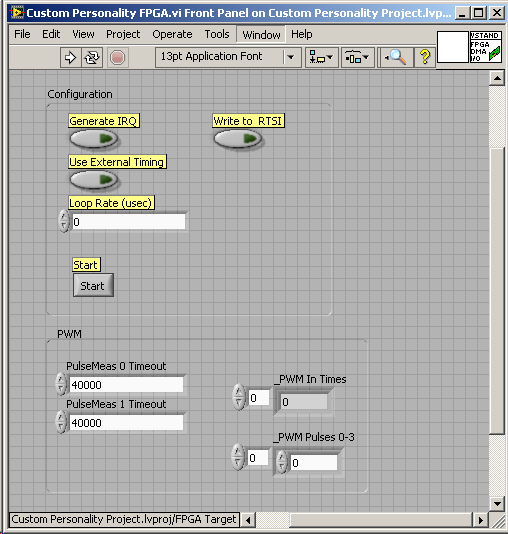
\includegraphics[scale=0.45]{Screenshots/Screenshot_2015-01-16_19-28-41.png}
	\caption{Create Labview FPGA target and XML - 10}
	\label{fig: Create Labview FPGA target and XML-10} 
\end{figure}
\begin{figure}[htb!]
	\centering 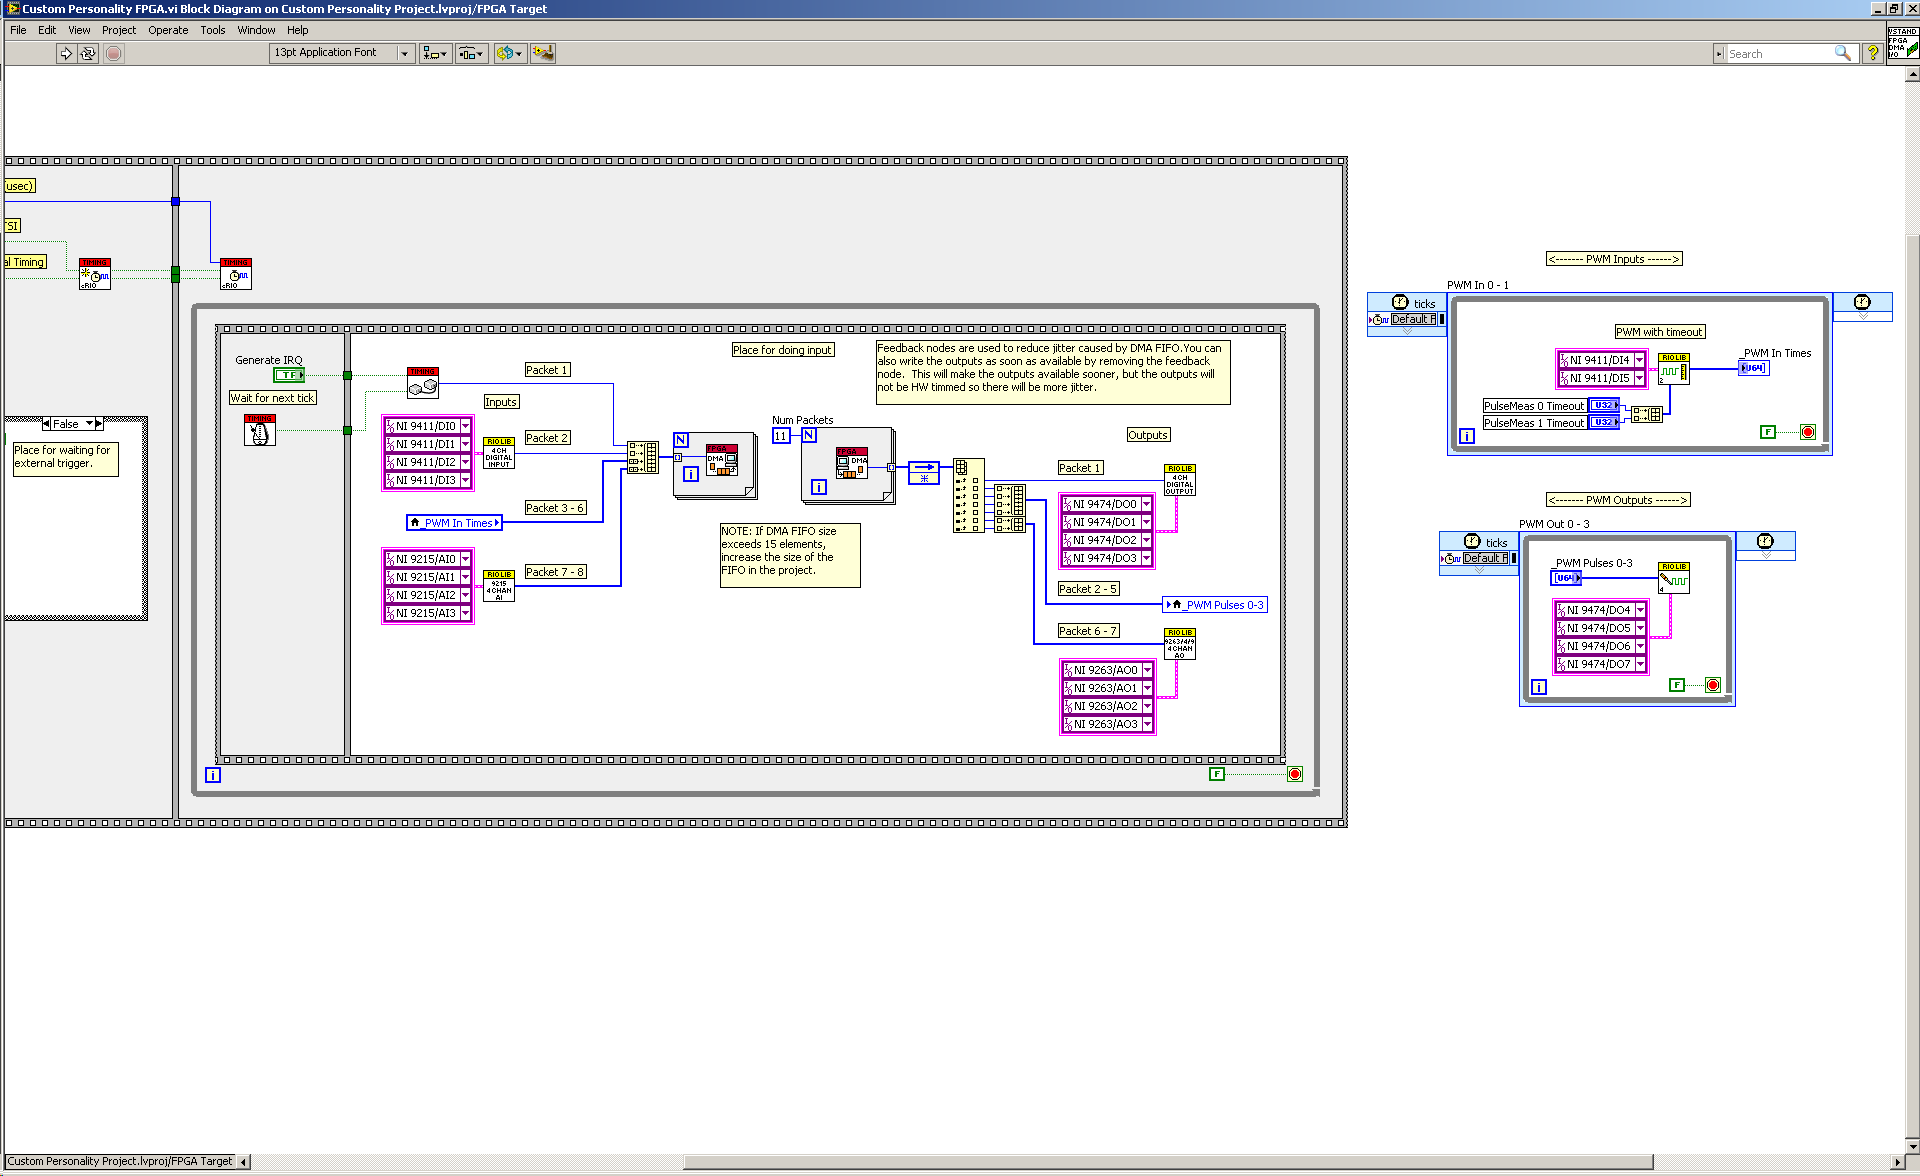
\includegraphics[angle=-90,scale=0.45]{Screenshots/Screenshot_2015-01-16_19-29-04.png}
	\caption{Create Labview FPGA target and XML - 11}
	\label{fig: Create Labview FPGA target and XML-11} 
\end{figure}
\begin{figure}[htb!]
	\centering 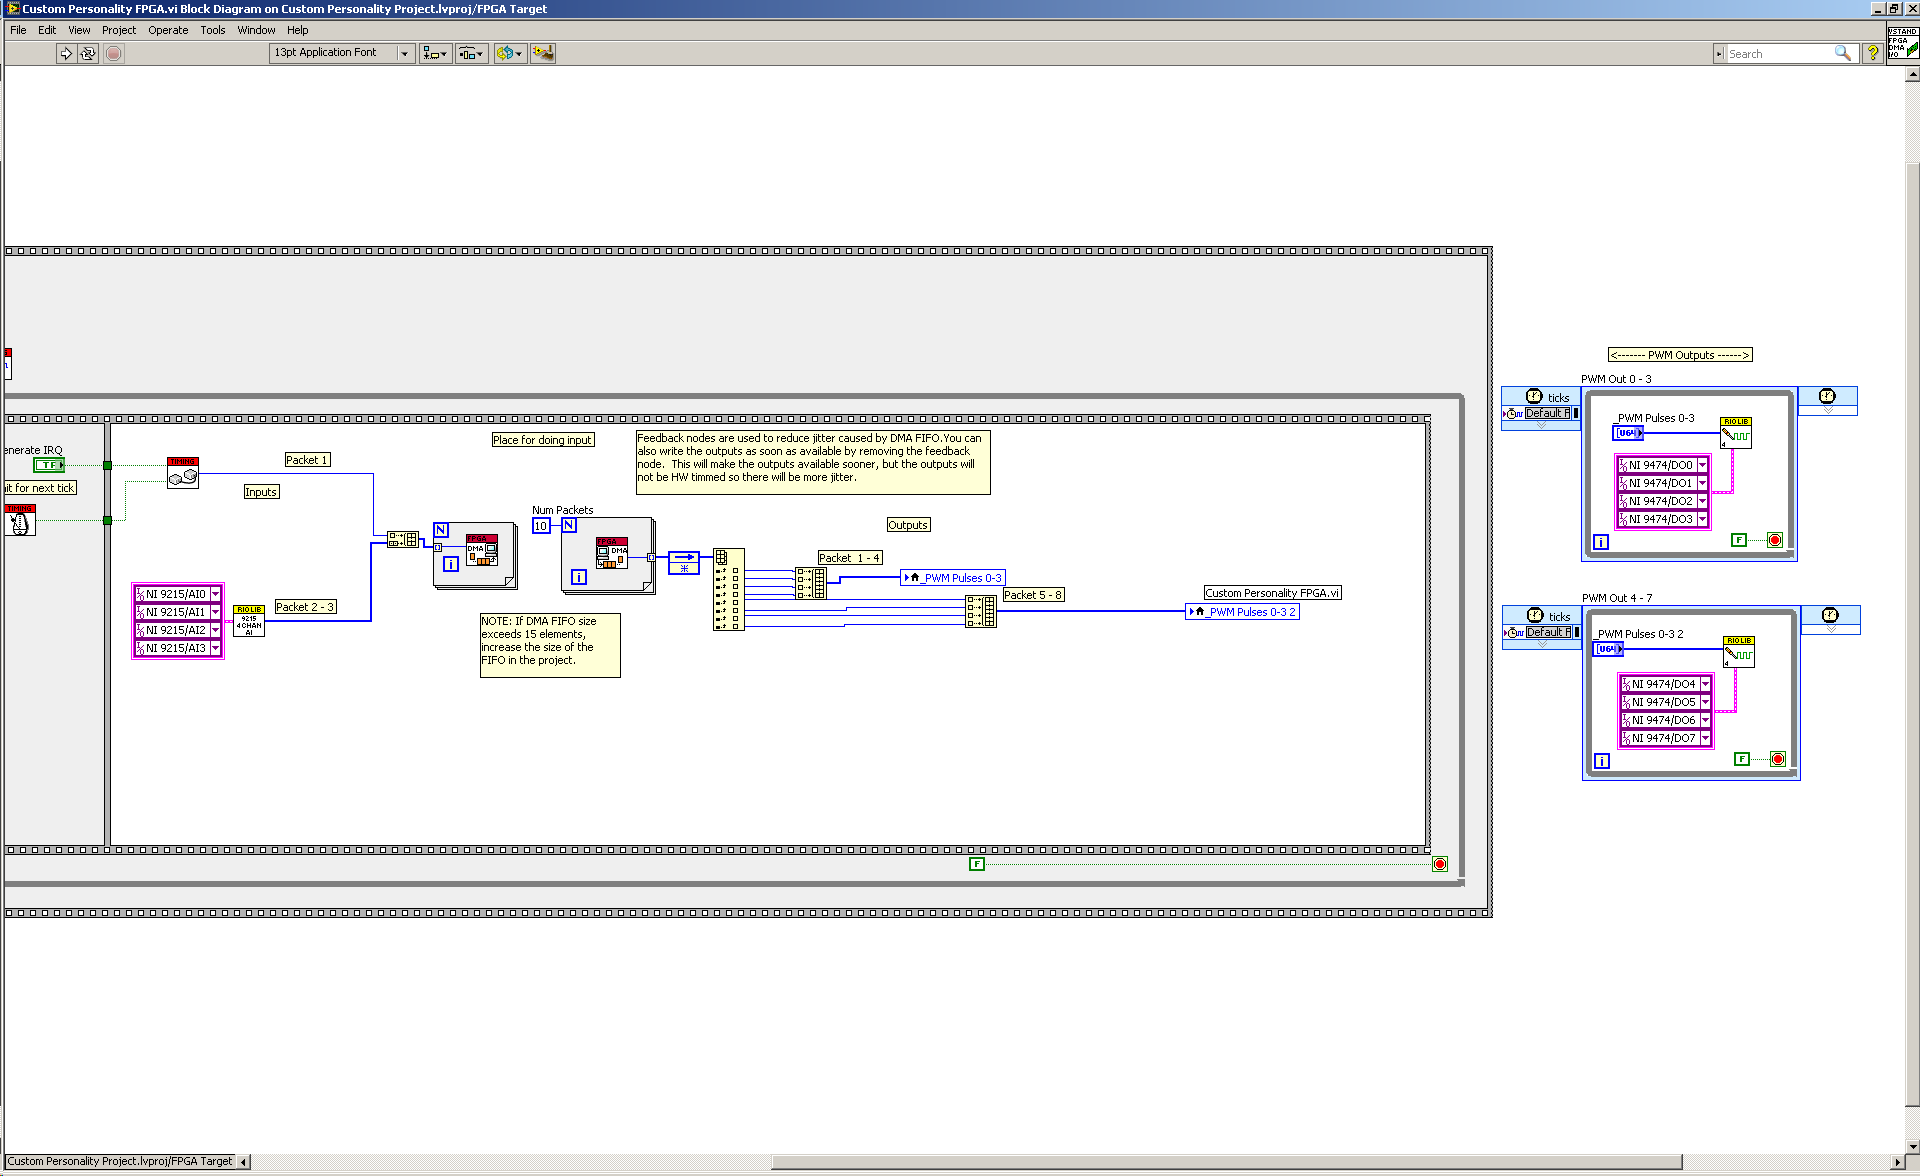
\includegraphics[angle=-90,scale=0.45]{Screenshots/Screenshot_2015-01-16_20-07-43.png}
	\caption{Create Labview FPGA target and XML - 12}
	\label{fig: Create Labview FPGA target and XML-12} 
\end{figure}
\begin{figure}[htb!]
	\centering 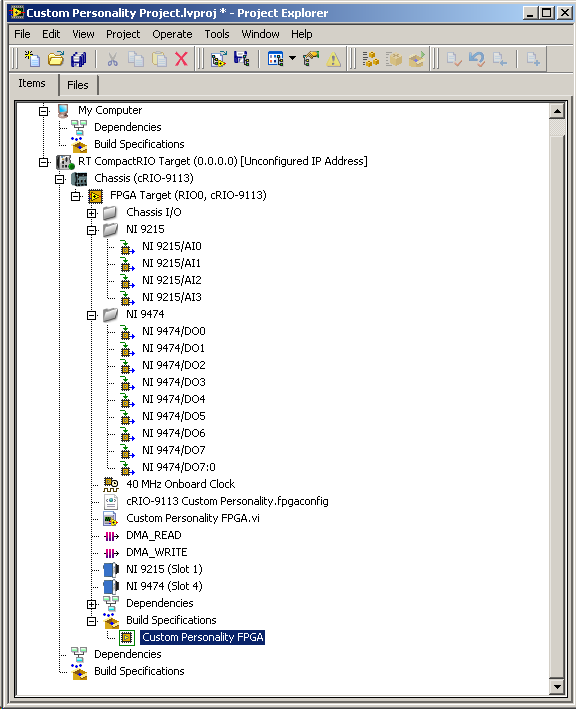
\includegraphics[scale=0.45]{Screenshots/Screenshot_2015-01-16_19-52-25.png}
	\caption{Create Labview FPGA target and XML - 13}
	\label{fig: Create Labview FPGA target and XML-13} 
\end{figure}
\begin{figure}[htb!]
	\centering 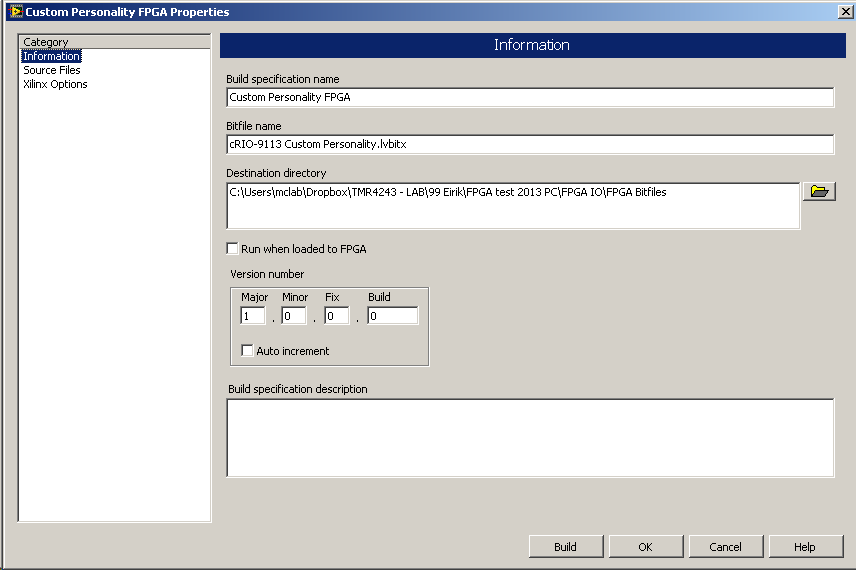
\includegraphics[scale=0.45]{Screenshots/Screenshot_2015-01-16_19-53-01.png}
	\caption{Create Labview FPGA target and XML - 14}
	\label{fig: Create Labview FPGA target and XML-14} 
\end{figure}
\begin{figure}[htb!]
	\centering 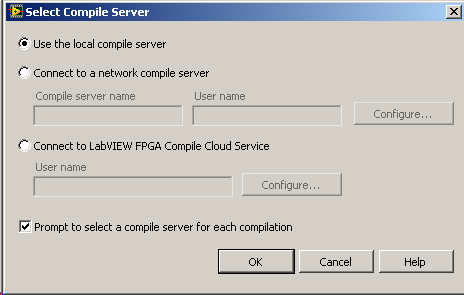
\includegraphics[scale=0.45]{Screenshots/Screenshot_2015-01-16_19-53-25.png}
	\caption{Create Labview FPGA target and XML - 15}
	\label{fig: Create Labview FPGA target and XML-15} 
\end{figure}
\begin{figure}[htb!]
	\centering 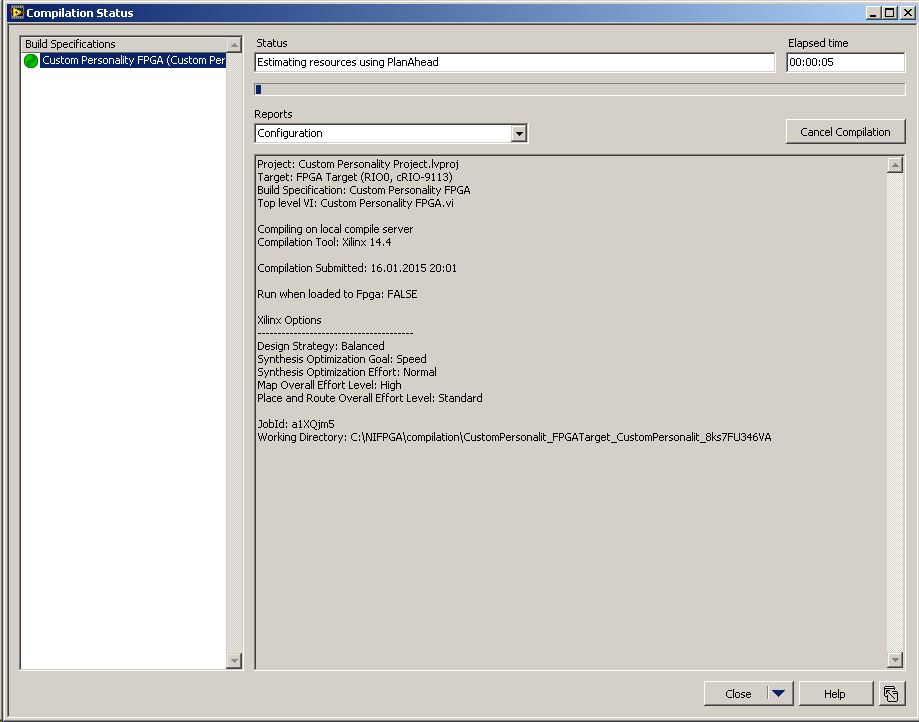
\includegraphics[scale=0.45]{Screenshots/Screenshot_2015-01-16_20-01-32.png}
	\caption{Create Labview FPGA target and XML - 16}
	\label{fig: Create Labview FPGA target and XML-16} 
\end{figure}
\begin{figure}[htb!]
	\centering 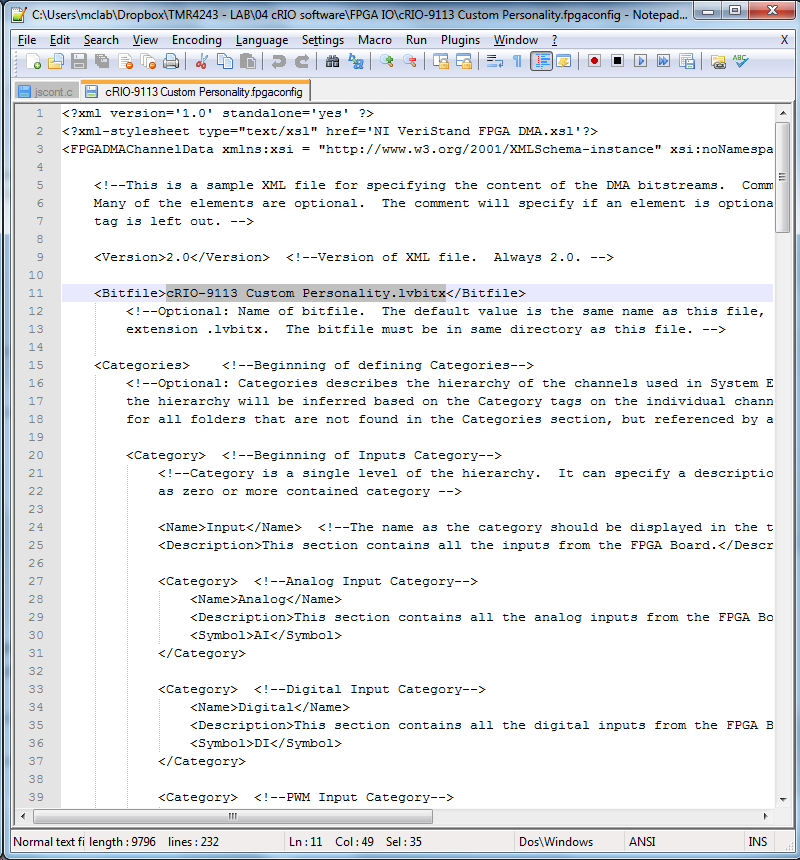
\includegraphics[scale=0.45]{Screenshots/Screenshot_2015-01-17_13-59-31.png}
	\caption{Create Labview FPGA target and XML - 17}
	\label{fig: Create Labview FPGA target and XML-17} 
\end{figure}

\subsection{Install in VeriStand}\label{sec:install_FPGA_in_veristand}

The Veristand software does not recognize the physical I/O components of the cRIO. It is necessarry to write a specific FPGA mapping for the specific setup. This results in a XML file that maps the ports. 

To add this file to your Veristand project, enter the system explorer and find the FPGA pane under \textit{targets\textbackslash{}controller\textbackslash{}hardware\textbackslash{}chassis}, as seen in Figure \ref{fig: fpga1}. 
\begin{figure}[htb!]
	\centering 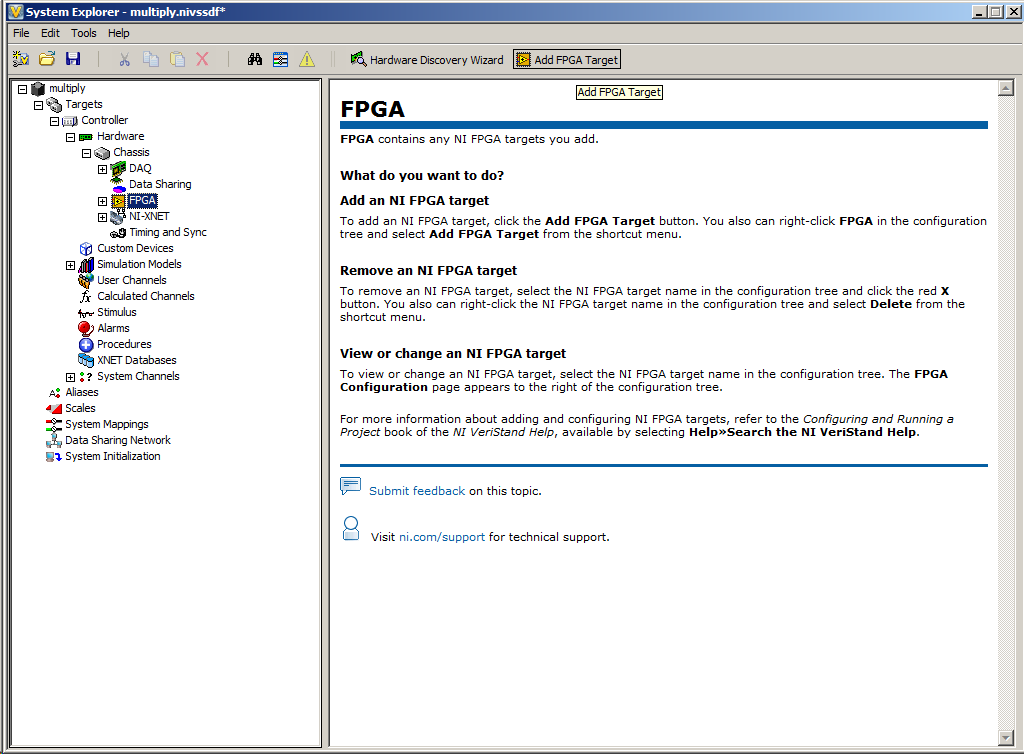
\includegraphics[scale=0.45]{fig/fpga1}
	\caption{FPGA1}
	\label{fig: fpga1}
\end{figure}
The next step is to find your XML file. In this case called cRIO-9113 Ex, it is very important that the XML file is placed on level above the FPGA bitfile folder in the directory system, as the files are really being used are the FPGA bitfiles.
\begin{figure}[htb!]
	\centering 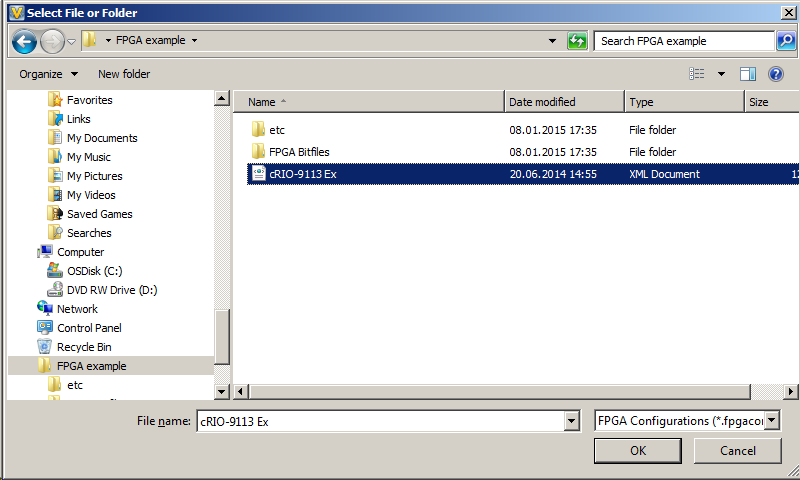
\includegraphics[scale=0.45]{fig/fpga2}
	\caption{FPGA2}
	\label{fig: fpga2}
\end{figure}
The menu in should now look something like Figure \ref{fig: fpga2}, here you can see the analogue input signals and the digital output PWM signals. These can again be linked to other signals as seen in Figure\ref{fig: veristand mappings}.
\begin{figure}
	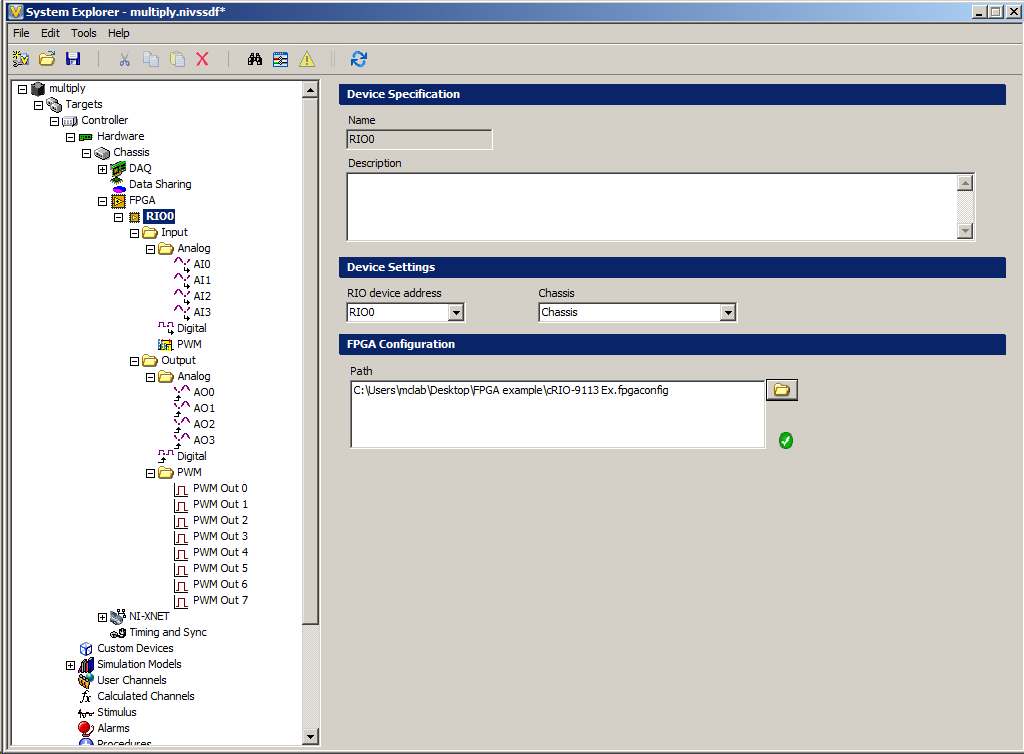
\includegraphics[scale=0.45]{fig/fpga3}
	\caption{FPGA3}
	\label{fig: fpga3}
\end{figure}
\subsubsection{Ticks}
tick = FPGA clock pulse
\[\text{tick in seconds}=\frac{1}{\text{frequency}}=\frac{1}{40MHz}=\frac{1}{40*10^{6}}=25*10^{-}9=25ns\]
output at 50 Hz demands output every 
\[\frac{40MHz}{50Hz}=\frac{40*10^{6}}{50}=800000tick\]
\section{Custom Device}
\subsection{Install}\label{subsec: Installing custom device driver}
As of July 2017, there are 3 different Custom Device drivers developed for use in MCLab: 
\begin{description}
	\item [WL\_Joystick] - used for reading sixaxis data sent from the RPi. Created by Torgeir Wahl
	\item [Oqus] - used for reading position and orientation data sent from the Qualisys system. Created by Torgeir Wahl
	\item [IMU] - used for reading IMU data from 4 IMU's, mainly intended for CSAD. Created by Guttorm Udjus
\end{description}
To install a Custom Device driver, the first step is to copy the folder with the driver to the path: \path{C:\Users\Public\Documents\National Instruments\NI VeriStand 201X\Custom Devices}
The directory should now contain something like Figure \ref{fig: custom device folder}.
\begin{figure}[htb!]
	\centering 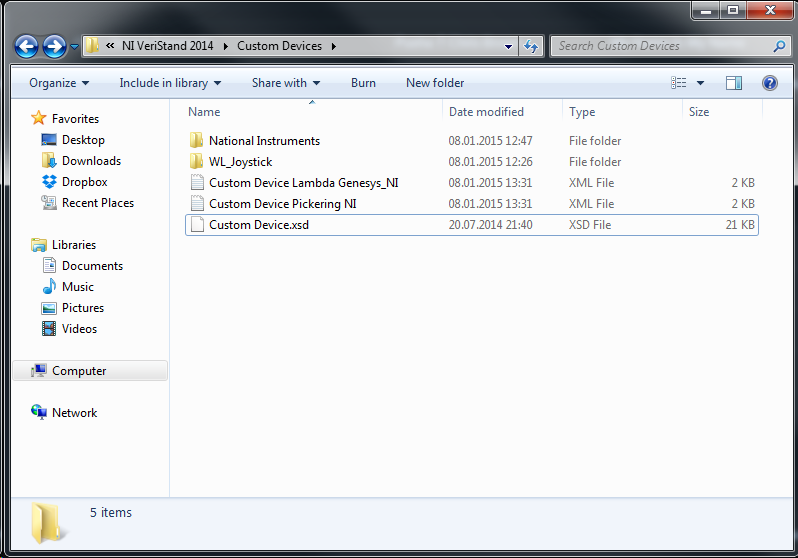
\includegraphics[scale=0.45]{fig/custom_devices_folder.png}
	\caption{Custom device folder}
	\label{fig: custom device folder} 
\end{figure}
The next step is to add custom device to your project. This is done in the system explorer, which is found as seen in Figure \ref{fig: veristand launch system explorer}.
\begin{figure}[htb!]
	\centering \includegraphics[scale=0.45]{fig/"veristand launch system explorer".png}
	\caption{VeriStand launch system explorer}
	\label{fig: veristand launch system explorer} 
\end{figure}
When in the system explorer, adding the custom device should be as simple as right clicking the custom device pane and choosing WL\_Joystick, as in Figure \ref{fig: custom device selection}. If you do not find the custom device WL\_Joystick, the most likely problem is that the placement of the custom device folder from step 1 is wrong.
\begin{figure}[htb!]
	\centering \includegraphics[scale=0.45]{fig/"veristand custom driver select".png}
	\caption{Custom device selection}
	\label{fig: custom device selection} 
\end{figure}
If the installation is successful you should be able to see WL\_Joystick folder under custom devices as seen in the red box in Figure \ref{fig: veristand confirmation}. Here you will also see the different inputs from the custom device, in this case it is joystick axis.
\begin{figure}[htb!]
	\centering \includegraphics[scale=0.45]{fig/"veristand mapping".png}
	\caption{VeriStand}
	\label{fig: veristand confirmation} 
\end{figure}
To connect the joystick to the input ports of the Simulink model. You open the system configuration mappings (click the button marked by the arrow in Figure \ref{fig: veristand confirmation}).
\begin{figure}[htb!]
	\centering \includegraphics[scale=0.45]{fig/"veristand mapping2".png}
	\caption{VeriStand System Configuration Mappings}
	\label{fig: veristand mappings} 
\end{figure}
You the simply find the ports you would like to connect, mark them and click the connect button. Figure \ref{fig: veristand mappings} a joystick output is connected to a input port on the Simulink model.
\section{Raspberry Pi}\label{subsec: RPi setup}
The unit is configured with Raspbian Linux-kernel-based operating system 
\subsection{Raspbian installation and setup}
This section describes how to install and access the Raspbian operating system on the RPi from a Windows computer. The operations are also possible from an OSX or Linux computer.
\subsubsection{Download operating system and utilities}
Download and extract the newest Raspbian\footnote{raspberrypi.org/downloads} operating system (OS) image. Necessary utilities for the setup are
\begin{itemize}
	\item Win32 Disk Imager\footnote{sourceforge.net/projects/win32diskimager} to write the OS image to the RPi SD card
	\item Advanced IP scanner\footnote{by Famatech, advanced-ip-scanner.com} to find the RPi address on the network 
	\item Putty terminal emulator\footnote{www.chiark.greenend.org.uk/\textasciitilde{}sgtatham/putty/download.html} for SSH connection
	\item WinSCP\footnote{by Martin Prikryl, winscp.net/eng/download.php} for file transfer
\end{itemize}
\begin{table}[h!]
	\centering
	\begin{tabular}{ll}
		\hline
		Windows & Linux, OSX\\
		\hline 
		Win32 Disk Imager & dd\\
		Advanced IP scanner & nmap\\
		Putty & ssh\\
		WinSCP & sftp\\
		\hline
	\end{tabular}
	\caption{RPi installation and setup utilities}
	\label{tab:RPi_utilities} 
\end{table}
See Table \ref{tab:RPi_utilities} for a list of the equivalent software for OSX and Linux.
\subsubsection{Write image to SD card}
Since the .iso file is raw, it needs to be written to the SD card in way that makes it bootable. Win32 Disk Imager does this.
\begin{figure}[htb!]
	\centering 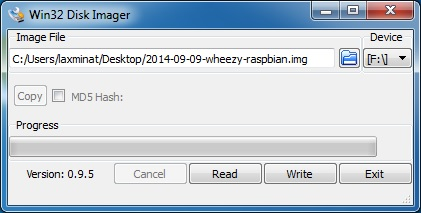
\includegraphics[scale=0.45]{fig/Rpi_DiskImager} \caption{Disk Imager}
	\label{fig: Disk Imager} 
\end{figure}
Run the program as administrator. Select the correct image file and device, as in Figure \ref{fig: Disk Imager}. Make sure that you have selected the correct drive before you push \texttt{Write}. Once the write is complete, insert the SD card in the RPi and boot.
\subsubsection{Terminal access}\label{subsec: Terminal access}
RPi can be accessed through the network, i.e. without having to directly connect a monitor and keyboard.
\begin{figure}[htb!]
	\centering 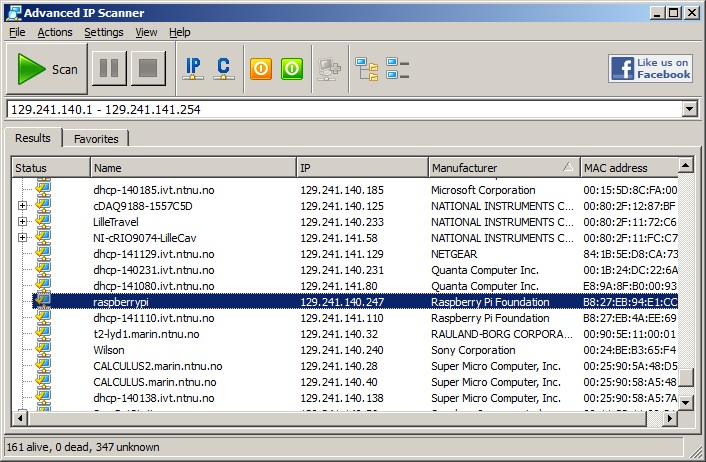
\includegraphics[scale=0.45]{fig/advancedIPscanner} \caption{Advanced IP Scanner}
	\label{fig: Advanced IP Scanner} 
\end{figure} 
At first boot, the RPi by default waits to be assigned an IP address by DHCP. If this address is not known, scan the network with Advanced IP Scanner. It is advicible to sort the results by manufacturer since it is fixed (\textit{Raspberry Pi Foundation}). The name is typically \emph{raspberrypi}. See Figure \ref{fig: Advanced IP Scanner}.
\begin{figure}[htb!]
	\centering 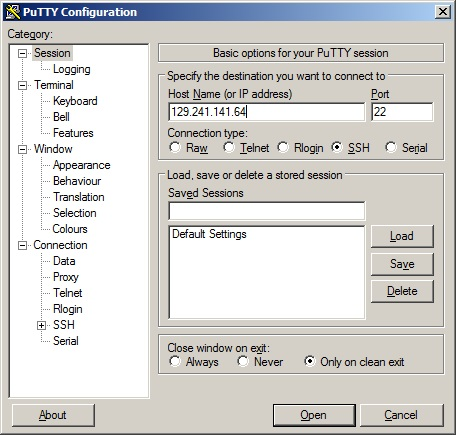
\includegraphics[scale=0.45]{fig/Rpi_remote_access1} \caption{Putty settings}
	\label{fig: Putty settings} 
\end{figure}
Once the IP is known, it is specified in the Putty settings, as in Figure \ref{fig: Putty settings}, and a connection can be opened. 
\begin{figure}[htb!]
	\centering 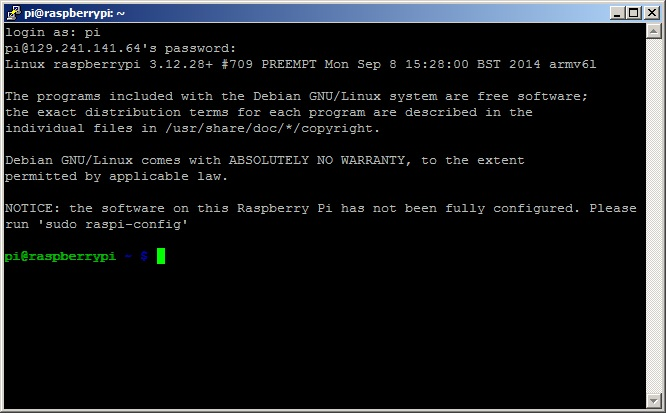
\includegraphics[scale=0.45]{fig/Rpi_remote_access2} \caption{SSH connection}
	\label{fig: SSH connection} 
\end{figure}
The default login is \texttt{pi}, and the default password \texttt{raspberry}. Figure \ref{fig: SSH connection} shows the terminal output on first login.
\subsubsection{Finalize configuration}
\begin{figure}[htb!]
	\centering 
	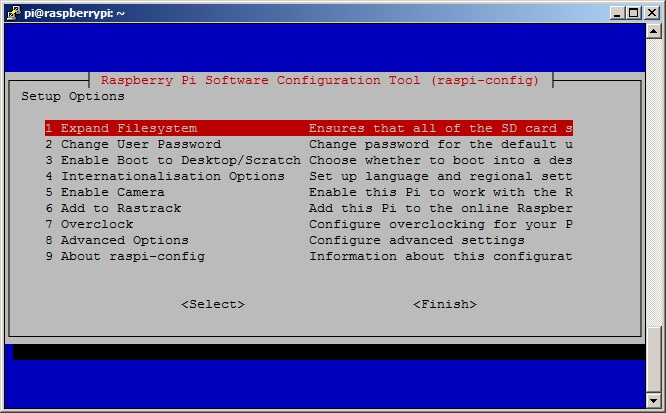
\includegraphics[scale=0.45]{fig/Rpi_finalize_install} 
	\caption{RPi configuration tool}
	\label{fig: RPi configuration tool} 
\end{figure}
Enter the\begin{verbatim}sudo raspi-config\end{verbatim}command to start the RPi Software Configuration Tool, as in Figure \ref{fig: RPi configuration tool}. Use the menu to apply the following
\begin{enumerate}
	\item Update configuration tool: 8 Advanced Options \textgreater  A9 Update
	\item Change password: 2 Change User Password
	\item Expand filesystem: 1 Expand Filesystem \textgreater  Finish
\end{enumerate}
Exit the configuration tool and select \texttt{Yes} for reboot. Reconnect through Putty.
Finally, update the repository package lists and upgrade all packages currently installed on the RPi:\begin{verbatim}sudo apt-get update 
sudo apt-get upgrade -y\end{verbatim}This process took approximately 10 minutes on a 90 Mbps internet connection. 
\subsubsection{Transfer files to RPi from computer}\label{subsec: Transfer files to RPi}
WinSCP can be used to transfer files to the RPi. This is useful for instance when transferring code, or when the RPi is not directly connected to the internet.
\subsubsection{Set fixed IP address}
When the RPi is connected directly to the cRIO or computer, a fixed IP is necessary since there is no DHCP server in that network. During most of this setup, however, it is preferable to keep the default DHCP assigned IP setting. To set a fixed IP
\begin{enumerate}
	\item Open the network interface configuration information file for editing\begin{verbatim}sudo nano /etc/network/interfaces\end{verbatim}
	\item Alter the eth0 settings from \texttt{dhcp} to \texttt{static} and
	add address and netmask as\begin{verbatim}auto eth0
	iface eth0 inet static
	address 192.168.1.22
	netmask 255.255.255.0\end{verbatim}
	\item Save the changes by the key combination \texttt{Ctrl+X}.
\end{enumerate}
The new IP is applied on the next reboot.

\subsection{Sixaxis installation and configuration}
This section describes how to install and configure the Sixaxis gamepad for Bluetooth connection to the RPi, and how to add a server for sending joystick signals to the cRIO.
\subsubsection{Download and install bluetooth support}
BlueZ is the official Linux Bluetooth stack. It provides support for core Bluetooth layers and protocols. To download and install, type
\begin{verbatim}sudo apt-get install bluez-utils bluez-compat bluez-hcidump
libusb-dev libbluetooth-dev joystick checkinstall -y\end{verbatim}
The process takes a few minutes.
\begin{figure}[htb!]
	\centering 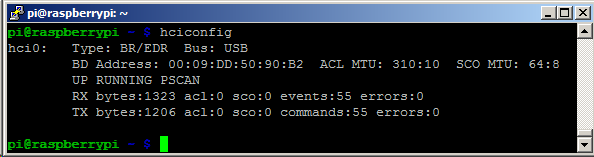
\includegraphics[scale=0.45]{fig/rpi_hciconfig} \caption{Bluetooth configuration tool}
	\label{fig: RPi hciconfig} 
\end{figure}
To confirm the installation, use the \texttt{hciconfig} command to print name and basic information about Bluetooth devices installed in the system. The output should include \texttt{UP RUNNING PSCAN}, as in Figure \ref{fig: RPi hciconfig}. If instead it says \texttt{DOWN}, some error har occured. Most experienced errors were due to typos.
\subsubsection{Bluetooth pairing}\label{par: Bluetooth-pairing}
Sixaxis does not support the standard Bluetooth paring prcedure, instead, pairing is done over USB. The \texttt{sixpair} command-line utility\footnote{by Pabr Technologies, www.pabr.org} searches USB buses for Sixaxis devices and tells them to connect to a new Bluetooth master.

Download and compile the program by the following commands:
\begin{verbatim}wget http://www.pabr.org/sixlinux/sixpair.c
gcc -o sixpair sixpair.c -lusb\end{verbatim}
Connect the Sixaxis by USB before running the paring utility
\begin{verbatim}sudo ./sixpair\end{verbatim}
The output should be similar to
\begin{verbatim}Current Bluetooth master: 00:02:72:BF:BC:8F
Setting master bd_addr to: 00:02:72:BF:BC:8F\end{verbatim}
The addresses at the end of each line will only be the same if you have already paired the Sixaxis with the Bluetooth dongle. First time they will be different. The Sixaxis USB cable may now be disconnected.

\subsubsection{Joystick manager system service}
\texttt{QtSixA}\footnote{the Sixaxis Joystick Manager by falkTX, qtsixa.sourceforge.net} reads the Sixaxis signals and makes them available to other programs. This program needs to run automatically whenever the RPi is booted.

To download the program, type
\begin{verbatim}wget http://sourceforge.net/projects/qtsixa/files/QtSixA%201.5.1/QtSixA-1.5.1-src.tar.gz\end{verbatim}
To install, type

\begin{verbatim}tar xfvz QtSixA-1.5.1-src.tar.gz
cd QtSixA-1.5.1/sixad
make
sudo mkdir -p /var/lib/sixad/profiles
sudo checkinstall -y\end{verbatim}
Update the system service list with sixad driver and reboot
\begin{verbatim}sudo update-rc.d sixad defaults
sudo reboot\end{verbatim}
To test the program, turn on the Sixaxis (round PS button in the middle) and start the test program
\begin{verbatim}sudo jstest /dev/input/js0\end{verbatim}
The terminal should now fill up with numbers that change as you move the analogue sticks and press the buttons on the Sixaxis. Exit the program by the key combination \texttt{Ctrl+C}.

\subsubsection{Joystick signal server}
A server must run to make joystick signals available over the RPi ethernet port. This should also start whenever the RPi is booted.

Transfer the source file \texttt{jscont.c} to the RPi (see Section
\ref{subsec: Transfer files to RPi}), then compile:

\begin{verbatim}g++ -o jscont jscont.c\end{verbatim}

To verify that the program runs correctly, turn off (hold PS3 button
for about 10 seconds) the previously paired Sixaxis and start the
program

\begin{verbatim}./jscont\end{verbatim}

\begin{figure}[h!]
	\centering 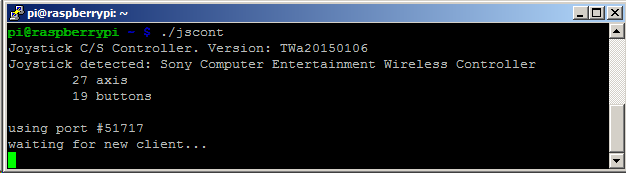
\includegraphics[scale=0.45]{fig/RPi_jscont} \caption{Joystick signal server test}
	\label{fig: RPi joystick server} 
\end{figure}

The program should then wait until you turn on the Sixaxis before
giving output simular to Figure \ref{fig: RPi joystick server}. To
exit the server use the key combination \texttt{Ctrl+C}.

Next, disable login at start-up in the bootup service description
\texttt{inittab}:
\begin{enumerate}
	\item Open the file for editing \begin{verbatim}sudo nano /etc/inittab\end{verbatim}
	\item Change the line that reads \begin{verbatim}1:2345:respawn:/sbin/getty --noclear 38400 tty1\end{verbatim}
	by adding \texttt{-{}-autologin pi} to get \begin{verbatim}1:2345:respawn:/sbin/getty --autologin pi --noclear 38400 tty1\end{verbatim}
	\textbf{Warning:} Typos here may result consequences hard to correct.
	\item Save and exit the changes by the key combination \texttt{Ctrl+X}.
\end{enumerate}
Finally, add \texttt{jscont} to the login execution file:
\begin{enumerate}
	\item Open the file for editing \begin{verbatim}sudo nano /home/pi/.bashrc\end{verbatim}
	\item At the very end of the file, add \begin{verbatim}sudo ./jscont\end{verbatim}
	\item Save the changes by the key combination \texttt{Ctrl+X}.
\end{enumerate}
RPi should now be sending joystick signals at start-up.